\documentclass[10pt,a4paper,landscape]{article}
\usepackage[margin=0.5in]{geometry}
\usepackage{amsmath,amssymb}
\usepackage{tikz}
\usetikzlibrary{shapes.geometric,arrows.meta,positioning,calc,fit,backgrounds}
\usepackage{times}

\newcommand{\pk}[1]{\textbf{#1}}
\newcommand{\idx}[1]{\textit{#1}}
\newcommand{\comp}[1]{\texttt{#1}}

\pagestyle{empty}

\begin{document}

\begin{center}
{\Large \textbf{4.5\quad Browser IndexedDB Architecture \& Database Schema (\texttt{PrismDB})}}\\[0.8em]

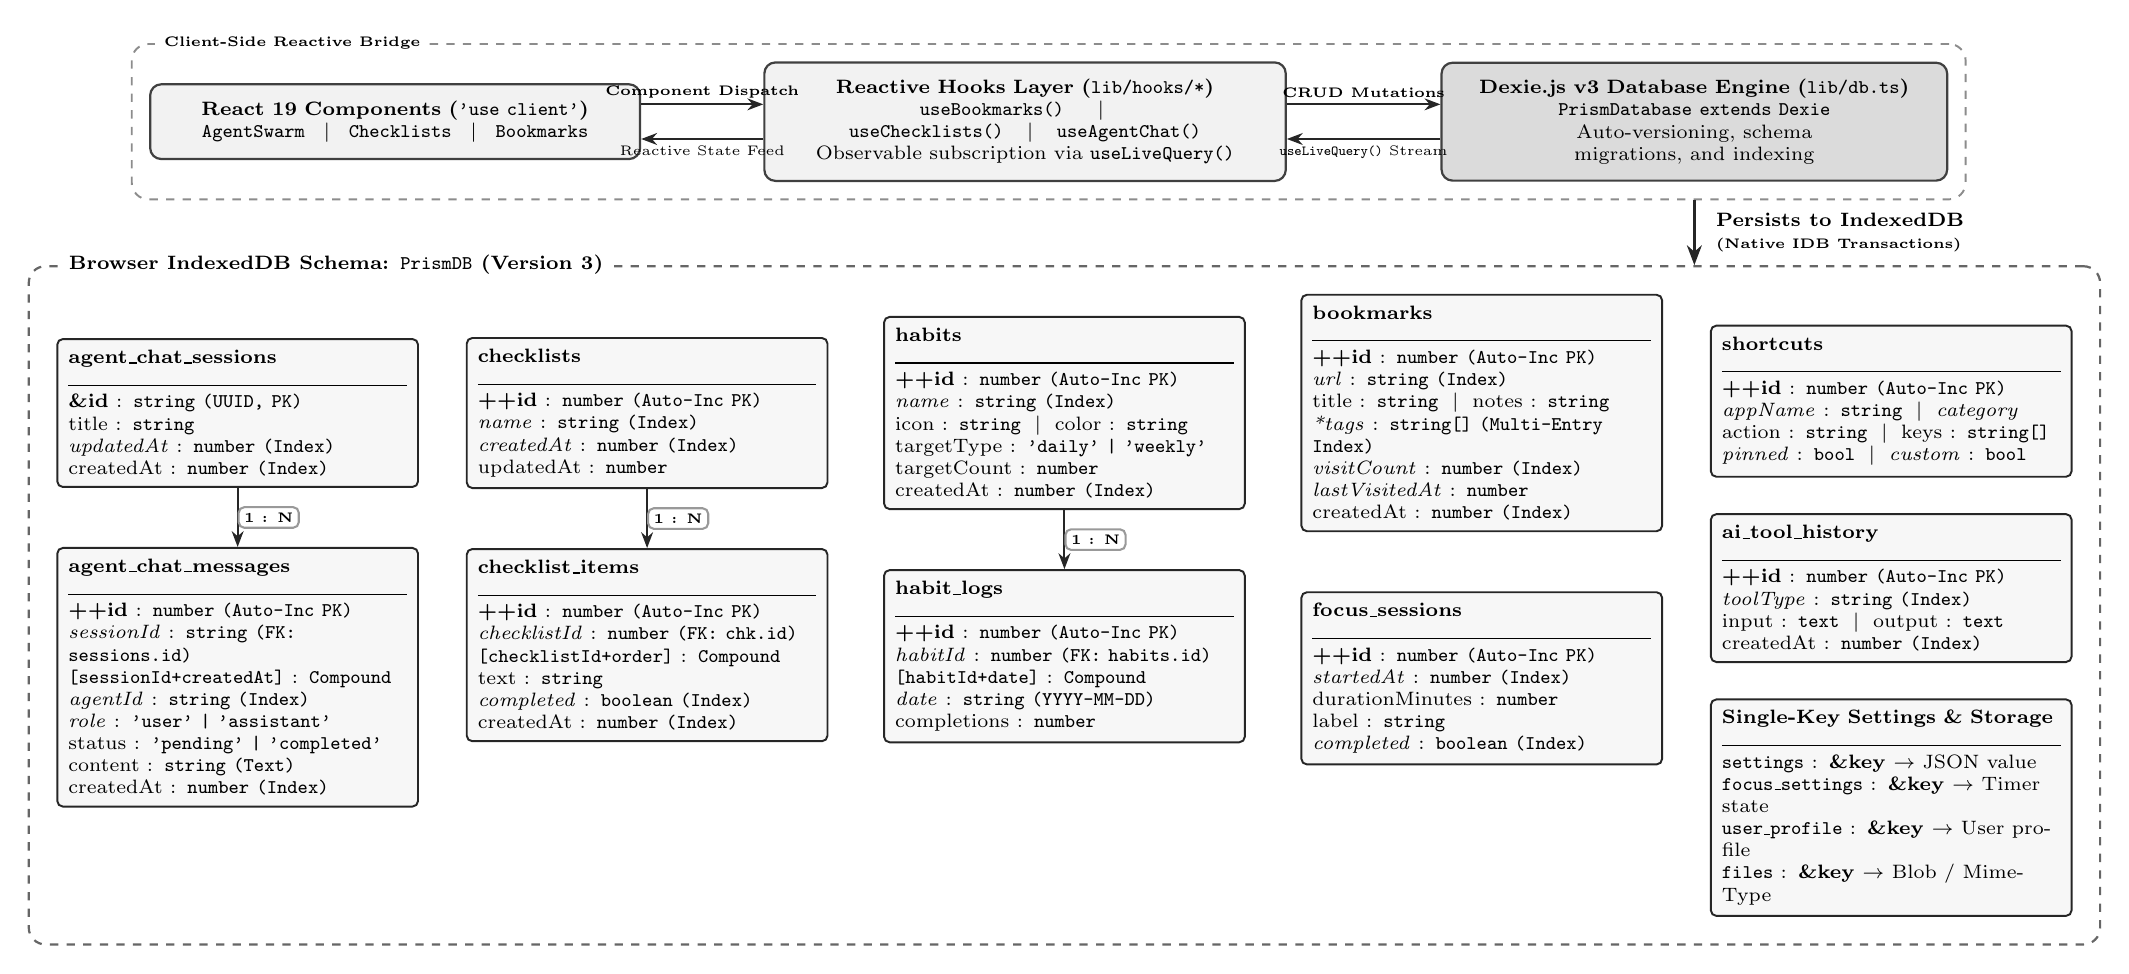
\begin{tikzpicture}[
    auto,
    font=\scriptsize,
    table/.style = {
        rectangle,
        draw=black!85,
        line width=0.7pt,
        fill=black!3,
        rounded corners=2pt,
        text width=4.3cm,
        inner sep=4pt
    },
    table_header/.style = {
        font=\scriptsize\bfseries,
        fill=black!18,
        draw=black!85,
        line width=0.6pt,
        text width=4.2cm,
        align=center,
        inner sep=3pt
    },
    system_box/.style = {
        rectangle,
        draw=black!75,
        line width=0.8pt,
        fill=black!5,
        rounded corners=4pt,
        inner sep=6pt,
        align=center
    },
    rel_arrow/.style = {
        -{Stealth[scale=0.9]},
        line width=0.75pt,
        draw=black!85
    },
    data_flow/.style = {
        -{Stealth[scale=0.85]},
        line width=0.65pt,
        dashed,
        draw=black!70
    }
]

    % =========================================================================
    % TOP: REACTIVE ARCHITECTURE FLOW
    % =========================================================================
    
    \node [system_box, text width=5.8cm] (react_ui) at (-8.5, 5.6) {
        \textbf{React 19 Components (\texttt{'use client'})}\\
        \texttt{AgentSwarm} $\;\vert\;$ \texttt{Checklists} $\;\vert\;$ \texttt{Bookmarks}
    };

    \node [system_box, text width=6.2cm] (hooks_layer) at (-0.5, 5.6) {
        \textbf{Reactive Hooks Layer (\texttt{lib/hooks/*})}\\
        \texttt{useBookmarks()} $\;\vert\;$ \texttt{useChecklists()} $\;\vert\;$ \texttt{useAgentChat()}\\
        Observable subscription via \textbf{\texttt{useLiveQuery()}}
    };

    \node [system_box, text width=6.0cm, fill=black!14] (dexie_engine) at (8.0, 5.6) {
        \textbf{Dexie.js v3 Database Engine (\texttt{lib/db.ts})}\\
        \texttt{PrismDatabase extends Dexie}\\
        Auto-versioning, schema migrations, and indexing
    };

    % Dual parallel reactive flow arrows with clean separate channels
    \draw [rel_arrow] ($(react_ui.east)+(0, 0.22)$) -- 
        node[above, font=\tiny\bfseries, inner sep=2pt]{Component Dispatch} ($(hooks_layer.west)+(0, 0.22)$);
    \draw [rel_arrow] ($(hooks_layer.west)+(0, -0.22)$) -- 
        node[below, font=\tiny, inner sep=2pt]{Reactive State Feed} ($(react_ui.east)+(0, -0.22)$);
        
    \draw [rel_arrow] ($(hooks_layer.east)+(0, 0.22)$) -- 
        node[above, font=\tiny\bfseries, inner sep=2pt]{CRUD Mutations} ($(dexie_engine.west)+(0, 0.22)$);
    \draw [rel_arrow] ($(dexie_engine.west)+(0, -0.22)$) -- 
        node[below, font=\tiny, inner sep=2pt]{\textbf{\texttt{useLiveQuery()}} Stream} ($(hooks_layer.east)+(0, -0.22)$);

    % Boundary box for IndexedDB Engine
    \node [draw=black!45, dashed, rounded corners=6pt, line width=0.7pt, fit=(react_ui) (hooks_layer) (dexie_engine), inner sep=0.22cm] (top_boundary) {};
    \node [anchor=west, font=\tiny\bfseries, fill=white] at ($(top_boundary.north west)+(0.3,0)$) {Client-Side Reactive Bridge};

    % =========================================================================
    % BOTTOM: RELATIONAL INDEXEDDB TABLES (PRISMDB)
    % =========================================================================

    % --- COLUMN 1: AGENT CHAT & TELEMETRY ---
    
    \node [table] (t_sessions) at (-10.5, 1.9) {
        \textbf{agent\_chat\_sessions}\\
        \rule{\linewidth}{0.4pt}
        \pk{\&id} : \texttt{string (UUID, PK)}\\
        title : \texttt{string}\\
        \idx{updatedAt} : \texttt{number (Index)}\\
        createdAt : \texttt{number (Index)}
    };

    \node [table, below=0.75cm of t_sessions] (t_messages) {
        \textbf{agent\_chat\_messages}\\
        \rule{\linewidth}{0.4pt}
        \pk{++id} : \texttt{number (Auto-Inc PK)}\\
        \idx{sessionId} : \texttt{string (FK: sessions.id)}\\
        \comp{[sessionId+createdAt]} : \texttt{Compound}\\
        \idx{agentId} : \texttt{string (Index)}\\
        \idx{role} : \texttt{'user' | 'assistant'}\\
        status : \texttt{'pending' | 'completed'}\\
        content : \texttt{string (Text)}\\
        createdAt : \texttt{number (Index)}
    };

    % Clean ERD cardinality badge
    \draw [rel_arrow] (t_sessions.south) -- node[draw=black!40, fill=white, rounded corners=2pt, inner sep=2pt, font=\tiny\bfseries]{1 : N} (t_messages.north);

    % --- COLUMN 2: CHECKLISTS & TASKS ---
    
    \node [table] (t_checklists) at (-5.3, 1.9) {
        \textbf{checklists}\\
        \rule{\linewidth}{0.4pt}
        \pk{++id} : \texttt{number (Auto-Inc PK)}\\
        \idx{name} : \texttt{string (Index)}\\
        \idx{createdAt} : \texttt{number (Index)}\\
        updatedAt : \texttt{number}
    };

    \node [table, below=0.75cm of t_checklists] (t_items) {
        \textbf{checklist\_items}\\
        \rule{\linewidth}{0.4pt}
        \pk{++id} : \texttt{number (Auto-Inc PK)}\\
        \idx{checklistId} : \texttt{number (FK: chk.id)}\\
        \comp{[checklistId+order]} : \texttt{Compound}\\
        text : \texttt{string}\\
        \idx{completed} : \texttt{boolean (Index)}\\
        createdAt : \texttt{number (Index)}
    };

    % Clean ERD cardinality badge
    \draw [rel_arrow] (t_checklists.south) -- node[draw=black!40, fill=white, rounded corners=2pt, inner sep=2pt, font=\tiny\bfseries]{1 : N} (t_items.north);

    % --- COLUMN 3: HABITS & TRACKING ---
    
    \node [table] (t_habits) at (0.0, 1.9) {
        \textbf{habits}\\
        \rule{\linewidth}{0.4pt}
        \pk{++id} : \texttt{number (Auto-Inc PK)}\\
        \idx{name} : \texttt{string (Index)}\\
        icon : \texttt{string} $\;\vert\;$ color : \texttt{string}\\
        targetType : \texttt{'daily' | 'weekly'}\\
        targetCount : \texttt{number}\\
        createdAt : \texttt{number (Index)}
    };

    \node [table, below=0.75cm of t_habits] (t_habit_logs) {
        \textbf{habit\_logs}\\
        \rule{\linewidth}{0.4pt}
        \pk{++id} : \texttt{number (Auto-Inc PK)}\\
        \idx{habitId} : \texttt{number (FK: habits.id)}\\
        \comp{[habitId+date]} : \texttt{Compound}\\
        \idx{date} : \texttt{string (YYYY-MM-DD)}\\
        completions : \texttt{number}
    };

    % Clean ERD cardinality badge
    \draw [rel_arrow] (t_habits.south) -- node[draw=black!40, fill=white, rounded corners=2pt, inner sep=2pt, font=\tiny\bfseries]{1 : N} (t_habit_logs.north);

    % --- COLUMN 4: BOOKMARKS, FOCUS & TOOLS ---
    
    \node [table] (t_bookmarks) at (5.3, 1.9) {
        \textbf{bookmarks}\\
        \rule{\linewidth}{0.4pt}
        \pk{++id} : \texttt{number (Auto-Inc PK)}\\
        \idx{url} : \texttt{string (Index)}\\
        title : \texttt{string} $\;\vert\;$ notes : \texttt{string}\\
        \idx{*tags} : \texttt{string[] (Multi-Entry Index)}\\
        \idx{visitCount} : \texttt{number (Index)}\\
        \idx{lastVisitedAt} : \texttt{number}\\
        createdAt : \texttt{number (Index)}
    };

    \node [table, below=0.75cm of t_bookmarks] (t_focus) {
        \textbf{focus\_sessions}\\
        \rule{\linewidth}{0.4pt}
        \pk{++id} : \texttt{number (Auto-Inc PK)}\\
        \idx{startedAt} : \texttt{number (Index)}\\
        durationMinutes : \texttt{number}\\
        label : \texttt{string}\\
        \idx{completed} : \texttt{boolean (Index)}
    };

    % --- COLUMN 5: CONFIGURATION & UTILITIES ---
    
    \node [table] (t_shortcuts) at (10.5, 2.05) {
        \textbf{shortcuts}\\
        \rule{\linewidth}{0.4pt}
        \pk{++id} : \texttt{number (Auto-Inc PK)}\\
        \idx{appName} : \texttt{string} $\;\vert\;$ \idx{category}\\
        action : \texttt{string} $\;\vert\;$ keys : \texttt{string[]}\\
        \idx{pinned} : \texttt{bool} $\;\vert\;$ \idx{custom} : \texttt{bool}
    };

    \node [table, below=0.45cm of t_shortcuts] (t_ai_tool) {
        \textbf{ai\_tool\_history}\\
        \rule{\linewidth}{0.4pt}
        \pk{++id} : \texttt{number (Auto-Inc PK)}\\
        \idx{toolType} : \texttt{string (Index)}\\
        input : \texttt{text} $\;\vert\;$ output : \texttt{text}\\
        createdAt : \texttt{number (Index)}
    };

    \node [table, below=0.45cm of t_ai_tool] (t_kv) {
        \textbf{Single-Key Settings \& Storage}\\
        \rule{\linewidth}{0.4pt}
        \texttt{settings} : \pk{\&key} $\rightarrow$ JSON value\\
        \texttt{focus\_settings} : \pk{\&key} $\rightarrow$ Timer state\\
        \texttt{user\_profile} : \pk{\&key} $\rightarrow$ User profile\\
        \texttt{files} : \pk{\&key} $\rightarrow$ Blob / MimeType
    };

    % Schema Container Boundary encompassing all 5 columns cleanly
    \node [draw=black!60, dashed, rounded corners=6pt, line width=0.8pt, 
           fit=(t_sessions) (t_messages) (t_checklists) (t_items) (t_habits) (t_habit_logs) (t_bookmarks) (t_focus) (t_shortcuts) (t_ai_tool) (t_kv), 
           inner sep=0.35cm] (schema_boundary) {};
    \node [anchor=west, font=\scriptsize\bfseries, fill=white] at ($(schema_boundary.north west)+(0.4,0)$) {Browser IndexedDB Schema: \texttt{PrismDB} (Version 3)};

    % Prominent, clear persistence arrow connecting Dexie engine directly through the channel
    \coordinate (persist_start) at (top_boundary.south -| dexie_engine.south);
    \coordinate (persist_end) at (schema_boundary.north -| dexie_engine.south);
    \draw [rel_arrow, line width=1.1pt] (persist_start) -- 
        node[right, font=\scriptsize\bfseries, align=left, xshift=4pt]{Persists to IndexedDB\\\tiny(Native IDB Transactions)} (persist_end);

\end{tikzpicture}

\vspace{0.8em}
{\normalsize \textbf{Figure 4.4: Browser IndexedDB Database Schema and Reactive Data Architecture (\texttt{PrismDB})}}
\end{center}

\end{document}
